% This is based on "sig-alternate.tex" V1.9 April 2009
% This file should be compiled with V2.4 of "sig-alternate.cls" April 2009
%
\documentclass{report}

\usepackage[english]{babel}
\usepackage{graphicx}
\usepackage{tabularx}
\usepackage{subfigure}
\usepackage{enumitem}
\usepackage{url}


\usepackage{color}
\definecolor{orange}{rgb}{1,0.5,0}
\definecolor{lightgray}{rgb}{.9,.9,.9}
\definecolor{java_keyword}{rgb}{0.37, 0.08, 0.25}
\definecolor{java_string}{rgb}{0.06, 0.10, 0.98}
\definecolor{java_comment}{rgb}{0.12, 0.38, 0.18}
\definecolor{java_doc}{rgb}{0.25,0.35,0.75}

% code listings

\usepackage{listings}
\lstloadlanguages{Java}
\lstset{
	language=Java,
	basicstyle=\scriptsize\ttfamily,
	backgroundcolor=\color{lightgray},
	keywordstyle=\color{java_keyword}\bfseries,
	stringstyle=\color{java_string},
	commentstyle=\color{java_comment},
	morecomment=[s][\color{java_doc}]{/**}{*/},
	tabsize=2,
	showtabs=false,
	extendedchars=true,
	showstringspaces=false,
	showspaces=false,
	breaklines=true,
	numbers=left,
	numberstyle=\tiny,
	numbersep=6pt,
	xleftmargin=3pt,
	xrightmargin=3pt,
	framexleftmargin=3pt,
	framexrightmargin=3pt,
	captionpos=b
}

% Disable single lines at the start of a paragraph (Schusterjungen)

\clubpenalty = 10000

% Disable single lines at the end of a paragraph (Hurenkinder)

\widowpenalty = 10000
\displaywidowpenalty = 10000
 
% allows for colored, easy-to-find todos

\newcommand{\todo}[1]{\textsf{\textbf{\textcolor{orange}{[[#1]]}}}}

% consistent references: use these instead of \label and \ref

\newcommand{\lsec}[1]{\label{sec:#1}}
\newcommand{\lssec}[1]{\label{ssec:#1}}
\newcommand{\lfig}[1]{\label{fig:#1}}
\newcommand{\ltab}[1]{\label{tab:#1}}
\newcommand{\rsec}[1]{Section~\ref{sec:#1}}
\newcommand{\rssec}[1]{Section~\ref{ssec:#1}}
\newcommand{\rfig}[1]{Figure~\ref{fig:#1}}
\newcommand{\rtab}[1]{Table~\ref{tab:#1}}
\newcommand{\rlst}[1]{Listing~\ref{#1}}

% General information

\title{Ripple BT - The future of local social networking\\
\normalsize{Distributed Systems -- Project Proposal}}
\subtitle{subtitle}

% Use the \alignauthor commands to handle the names
% and affiliations for an 'aesthetic maximum' of six authors.

\numberofauthors{1} %  in this sample file, there are a *total*
% of EIGHT authors. SIX appear on the 'first-page' (for formatting
% reasons) and the remaining two appear in the \additionalauthors section.
%
\author{
% You can go ahead and credit any number of authors here,
% e.g. one 'row of three' or two rows (consisting of one row of three
% and a second row of one, two or three).
%
% The command \alignauthor (no curly braces needed) should
% precede each author name, affiliation/snail-mail address and
% e-mail address. Additionally, tag each line of
% affiliation/address with \affaddr, and tag the
% e-mail address with \email.
%
% 1st. author
\alignauthor \normalsize{Carl Friess, Isaak Hanimann, Sven Knobloch, Laurin Paech,  Sebastian Winberg, David Yenicelik}\\
	\affaddr{\normalsize{cfriess  15-943-111, isaakh 15-913-312, knsven 14-945-166, lpaech 15-944-242, winbergs 15-941-222,  yedavid 15-944-366}}\\
	\email{\normalsize{cfriess@student.ethz.ch, isaakh@student.ethz.ch, knsven@student.ethz.ch, lpaech@student.ethz.ch, winbergs@student.ethz.ch, yedavid@student.ethz.ch}}
}


\begin{document}

\maketitle

\begin{abstract}
We propose a social networking application for sharing photos in close physical proximity, utilizing a combination of the Bluetooth Low Energy and BitTorrent protocols, as well as a custom RESTful HTTP API.

A user can take a picture, which is then broadcasted to all phones that are in the direct vicinity and part of the network.

The application uses the Bluetooth Low Energy Protocol for close proximity device discovery and messaging. However, the fundamental transfer of image files leverages peer-to-peer technology to reduce operational costs and increase performance. 

Every device runs a BitTorrent client, which seeds images it has already downloaded to other nodes within the network. The discovery of seeding devices is provided by a central BitTorrent tracker.

Another centralized server further allows devices to share torrent files, enabling the use of the BitTorrent protocol.

Our goal is to build a fully-working prototype with the proposed architecture.
\end{abstract}

\section{Introduction}

We first introduce two definitions:

\begin{enumerate}
\item \textbf{ripple} \textit{(noun)}: A message consisting of a photo that is being broadcasted to anyone nearby from a person's smartphone. 
\item \textbf{to ripple} \textit{(verb)}: When person A broadcasts a ripple. If a person B decides to share it again, the photo is 're-rippled'.
\end{enumerate}

\subsection{Problem Statement and Motivation}
There are numerous social networks, such as Instagram and Snapchat, that allow users to share moments with a specific group of people.
These services are often criticized for removing the personal element from social communication, because users are sitting behind screens or using their phones, rather than actually spending time together.

Our approach to social networking is to augment social interaction, rather than redefining and possibly inhibiting it. Social Networks should help form connections between people and not just build on existing ones.

\subsection{Concept}
Considering the above problem statement, we propose \textit{Ripple BT}: a social network that allows users to share moments with other users in their close proximity. The social network will consist of a freely available Android application with a focus on photos.

After a user takes a picture, it is broadcasted to all other users of the app in their immediate vicinity, regardless of their affiliation with the broadcasting user. Communication is, in principle, anonymous (disregarding content) and always public.

Users receiving broadcasted images may view them once. They are then presented with the choice of either simply discarding the image or instead rebroadcasting (\textit{re-rippling}) it to other users in their proximity.
Each user can view the ripple only once regardless of the number of re-ripples near them.

We believe this social network will encourage social interaction, as the communication can only take place when users are close to each other. Furthermore, the network allows interesting content to propagate, making it possible to share memorable moments in a wider radius.

\subsection{Application Scenario}
We will demonstrate a typical use case of the Android application in a group of people attending an event: \textit{Alice}, \textit{Bob}, \textit{Charlie} and \textit{Daniel}.

Alice takes a funny photo of a particular activity at the event and wants to raise awareness of the activity with other attendees. She therefore uses Ripple to share the image.

Bob, who is not far away receives the ripple and is intrigued by the picture. He thinks others might share his intrigue and re-ripples the image.

Charlie and Daniel are in close proximity of Bob but not of Alice. As Bob is also broadcasting the image and they have the Ripple app installed, they now also receive the ripple.

Following this scheme the ripple spreads out and propagates, maybe even beyond the event's location.

\subsection{Background}
This concept is related to an iOS application \cite{rippleDevpost} developed at the START Hack hackathon in March 2017. It is a basic implementation of this concept using Amazon S3 to store images, so they can be downloaded by the receiving devices. Bluetooth Low Energy is used to advertise images by setting the value of a well known GATT characteristic to the UUID of the image in the S3 bucket.

While this implementation works, it has several flaws. Firstly, uploading every image to an Amazon S3 bucket means that operation costs for storage are bound to be high without heavy compression.

Similarly, repeatedly downloading the image from one central point, causes high bandwidth consumption and possibly unnecessary data transfer costs.

Beyond this, the method for announcing ripples is also suboptimal. It does not work well, when a user would like to broadcast multiple ripples in quick succession and (on iOS) does not fully work when the application is in the background.

With Ripple BT we aim to redesign the system from the ground up with a focus on spreading the load of sending images among user devices, thus reducing operating costs and improving performance.

\begin{figure}[h]
	\centering
    \includegraphics[width=\columnwidth]{rippleslide.png}
    \lfig{example}
    \vspace{-5mm} % use negative white space to fix too large gaps
	\caption{Screenshots from the original Ripple application. Includes a view to take photos (left), a list of all received photos (middle), and an image viewer for received ripples (right)}
\end{figure}

\newpage

\subsection{Challenges}
This project has two main distributed challenges:
\begin{enumerate} 
    \item Finding users in close proximity
    \item Sending the image data
\end{enumerate}

For the first challenge of user discovery we investigated using GPS data to track the user location. Since GPS has a fairly weak accuracy with uncertainties as high as a few hundred meters when inside a building, we couldn't achieve sufficient locality using this technology. We therefore turned our focus to Bluetooth Low Energy. The range of 10-20 meters is optimal considering the desired behavior and less power consuming than GPS. Furthermore Bluetooth Low Energy provides a well established protocol with wide-spread hardware compatibility.

We considered the following aspects for the second challenge of sending the image data.
It became clear early on that Bluetooth Low Energy would not have high enough data rates to send an entire image from one device to another in a reasonable time frame and acceptable reliability. For this reason we first looked into a centralized structure (using Amazon S3) where images are stored with a UUID and the UUID is sent to the receiver over Bluetooth. The image can then be retrieved from the central server using the UUID.

While this implementation works, storage and bandwidth costs especially for a later support of video files would be fairly high. With the intentions of shifting most of the load to user devices and not storing the image data on a central server we looked into peer-to-peer technology. We considered the use of \textit{IPFS} \cite{ipfs} but decided to use the BitTorrent file sharing protocol since it is well established and commonly used with a large amount of software support.

With BitTorrent the devices can distribute the content amongst themselves. However, this requires a torrent file, leading to the question of how to send this file to other devices. Our first idea was to send the torrent file over Bluetooth Low Energy. But since torrent files can have a significant size themselves and BLE only allows for low data rates, we chose to only pass an identifier over Bluetooth and retrieve the torrent file from the central server using a custom RESTful HTTP API. Since one torrent file is only a few kilobytes in size, we have significantly lowered the cost by several orders of magnitude..


\section{System Overview}

\subsection{System Architecture}
To increase speed and reduce operating costs, the Android application does not solely rely on high-bandwidth connections with a centralized server, but rather uses a distributed peer-to-peer network to transmit photos between individual nodes.

The fundamental transfer of image files is done using BitTorrent. A central tracker will facilitate the discovery of nodes in accordance with the BitTorrent protocol. A receiving node will then download the image form the initial node and from other nodes, which have already completed the download.

A centralized server further allows devices to retrieve torrent files, which are necessary in the BitTorrent protocol.

Devices use the Bluetooth Low Energy Protocol for close proximity device discovery and for transmitting identifying information of  the broadcasted images.

\begin{figure}[h]
	\centering
    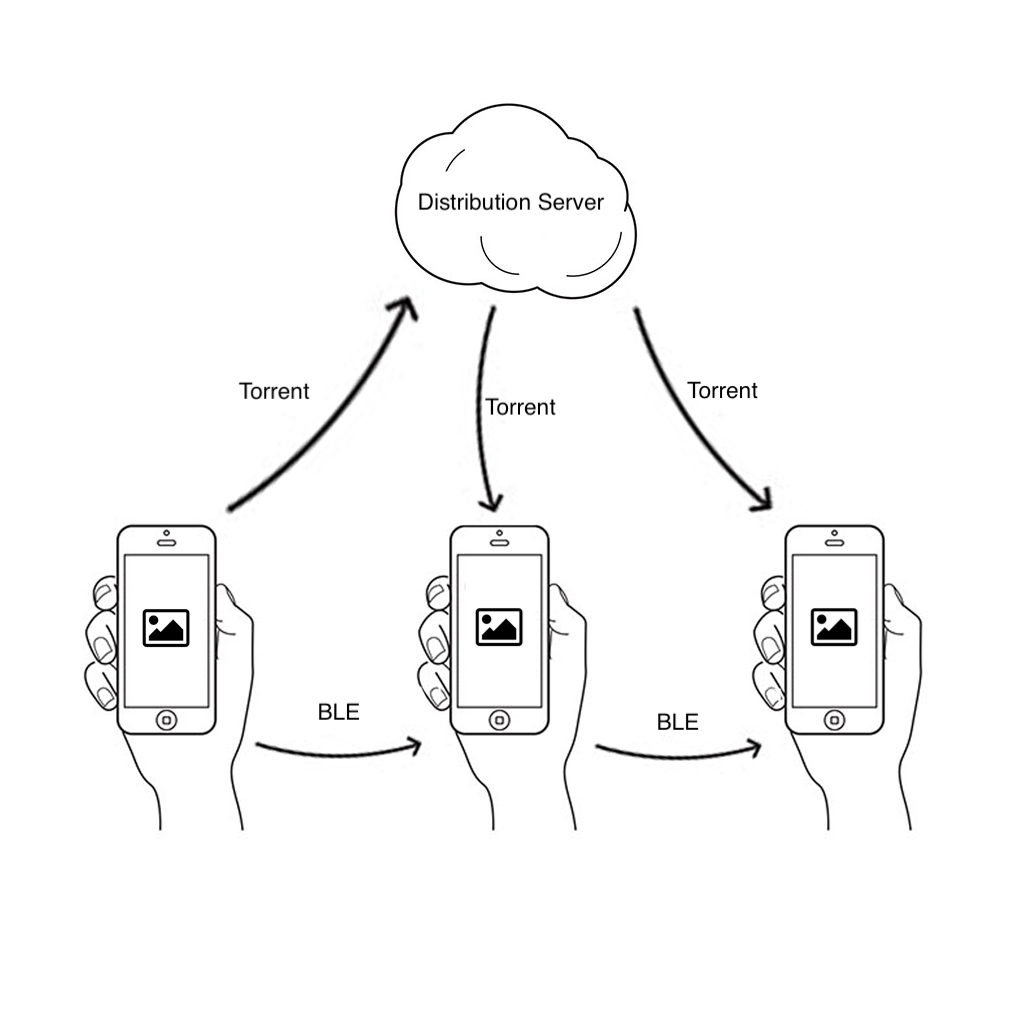
\includegraphics[width=\columnwidth]{overview.jpg}
    \lfig{system-overview}
    \vspace{-5mm} % use negative white space to fix too large gaps
	\caption{System Overview}
\end{figure}

\subsection{BitTorrent File Transfer}
Image files, which make up the largest portion of the data traffic, are transferred between devices peer-to-peer using the BitTorrent protocol.

We will use the \textit{ttorrent} library \cite{ttorrentLink}, a Java implementation of the BitTorrent protocol. With the help of this library, every device will run a BitTorrent client in an Android Service.

Each phone seeds all images it creates and receives for 24 hours. This way many seeding devices should become available quickly allowing for the load to be shared effectively. Furthermore, there is no need for any device or server to store the full image file indefinitely.

The BitTorrent protocol relies on a central tracker to let clients know which other clients are seeding the file. We chose to use the JavaScript \textit{bittorrent-tracker} library \cite{bittorrentTrackerLink} to achieve this functionality. The tracker will run on an \textit{Amazon EC2} \cite{ec2} instance.

\newpage

\subsection{Distribution of Torrent Files}
One of the challenges that we face is the limited data rates of the Bluetooth Low Energy protocol.

This leads to the issue that we can't transmit torrent files via Bluetooth Low Energy. Instead we have decided to use a distribution server, which associates torrent files with UUIDs.

Before broadcasting a new Ripple to other devices, the application uploads the torrent file for the image to the distribution server by means of a HTTP POST request. The server stores the torrent file in a \textit{MySQL} \cite{MySQLLink} database and returns a UUID. 

To retrieve a torrent file, the application submits an HTTP GET request containing the UUID. The server verifies the UUID by looking it up in a database and returns the corresponding torrent file. The application can then use it to invoke the BitTorrent protocol and download the associated image file.

\subsection{Bluetooth Low Energy}
For the advertisement of ripples we will use the Bluetooth Low Energy protocol as follows:

Each device will have a well known GATT service for ripples. In this service there is a well known characteristic that stores a sequence number. In addition, the service will have a characteristic for each ripple it is currently advertising. The UUID of that characteristic is used to query the torrent file from the central server.

The application is constantly scanning for devices with the Ripple GATT service and connects to them automatically.

If a device wants to send/broadcast a ripple, it adds a characteristic with the respective UUID to the Ripple GATT service and increments the value of the sequence number characteristic. This will notify connected devices of potential changes and the existence of a new ripple. The receiving device will then scan for new characteristics and proceed to retrieve the image for the ripple.

\subsection{Local SQLite Database}
The application needs to track information about the ripples it creates and receives. Primarily, the application concept only allows users to receive and view ripples once, so the application must be able to check for duplicates. Furthermore, the embedded BitTorrent client should only seed ripples for 24 hours, which will be ensured by storing the time frame in a database.
We have chosen to use an \textit{SQLite} \cite{sqliteLink} database for this task, as it provides all necessary features with good performance, while being easily embeddable in the application.

\section{Requirements}

\subsection{Hardware}
As this is a social networking application, we want to ensure that there are no hardware dependencies beyond a typical Android smartphone.

\subsection{Software (libraries and frameworks)}
We plan on using the following libraries and frameworks in the application:
\begin{itemize}
  \item \textbf{SQLite} \cite{sqliteLink} will be used as a local database to store information about ripples on the devices.
  \item \textbf{ttorrent} \cite{ttorrentLink} is a Java implementation of the BitTorrent protocol, which we will use to implement the embedded BitTorrent client in the application.
  \item The BitTorrent tracker implementation will be provided by the JavaScript \textbf{bittorrent-tracker} \cite{bittorrentTrackerLink} framework.
  \item The distribution server will be implemented in JavaScript and run in a \textbf{node.js} \cite{nodejsLink} environment.
  \item A \textbf{MySQL} \cite{MySQLLink} will store all torrent files on the distribution server. 
  \item We also utilize the \textit{UUID v6} standard to generate unique identifiers.\end{itemize}

\subsection{Third-party party services}
We also intend on using an Amazon EC2 instance to host the tracker and distribution server.
This instance has free plans for evaluation usage sufficient for our needs at the moment.

\section{Work Packages}
We identified and divided the project into the following work packages: 

\begin{itemize}
    \item {\bf WP1 - BitTorrent Client}: Implementing the management of the embedded BitTorrent Client.
    \item {\bf WP2 - Distribution Server}: Implementing a RESTful API for torrent file distribution.
    \item {\bf WP3 - Camera UI}: Implementing the camera and photo capture functionality of the app using the Android API.
    \item {\bf WP4 - Receive UI}: Implementing the receive stack of ripples including the re-ripple and discard functionality.
    \item {\bf WP5 - BLE Sending}: Implementing the sending/broadcasting of ripples via Bluetooth Low Energy.
    \item {\bf WP6 - BLE Receiving}: Implementing the receiving and scanning of ripples via Bluetooth Low Energy.
    \item {\bf WP7 - Local Database}: Implementing an interface to a local SQLite database for the storage of send and received ripples.
\end{itemize}

Each working package is intended to be done by an individual team member. Due to the dependencies of some of the packages it is necessary for certain group members to work together. Since some work packages are more extensive than others, team members are encouraged to help their fellow team mates when done with their own part. In the later stages of the project more and more interaction will be required in order to have a working and coherent application for the final submission. 
 
\section{Milestones}

We plan to uphold the following schedule:
\begin{itemize}
\item  \textbf{24. Nov. 2017}: First working versions of the individual work packages
\item  \textbf{4. Dec. 2017}: Integrated all work packages into one coherent working app
\item \textbf{8. Dec. 2017}: Tested application on multiple nodes, identifying bugs and generally debugging the system
\item \textbf{14. Dec. 2017}: Finished presentation and Ripple BT logo
\item \textbf{15. Dec. 2017}: Deadline for submission of presentation slides and project logo
\item \textbf{16. Dec. 2017}: Finished debugging entire system and fully working version of the app
\item \textbf{17. Dec. 2017}: Deadline for submission of code
\item \textbf{18. Dec. 2017}: Presentation and demo of project
\end{itemize}


\bibliographystyle{abbrv}
\bibliography{report}  % sigproc.bib is the name of the Bibliography in this case
% You must have a proper ".bib" file

\end{document}
